\section{Example}
\label{subsec:example}
%Step-by-step example (intention is to move this to an appendix)
Here, a contrived Hamiltonian is used to show the step-by-step procedure of LOBE. The example Hamiltonian, with a bosonic occupancy cutoff $\Omega = 3$, that will be used is 

\begin{equation}
    \label{ex}
    H = b_0^\dagger d_0(a_0^\dagger)^2 + 2 d_0^\dagger a_0^\dagger a_0+3 b_0^\dagger d_0^\dagger d_0
\end{equation}

\textbf{Step 1: Rescale Hamiltonian from bosonic terms:}
To rescale the coefficients of the Hamiltonian due to the presence of bosonic operators, equation \ref{bose coeff rescale}, is used. If we let $\alpha_0 = 1, \alpha_1 = 2, \alpha_2 = 3$, we obtain  $\alpha_0^* = 1,\alpha_1^* = 2, \alpha_2^* = 0.75$ since $K = 2$. Thus,
\begin{equation}
    \tilde{H} = b_0^\dagger d_0(a_0^\dagger)^2 + 2 d_0^\dagger a_0^\dagger a_0+0.75 b_0^\dagger d_0^\dagger d_0
\end{equation}

\textbf{Step 2: Rescale coefficients of Hamiltonian:} In order to load the Hamiltonian coefficients into the circuit via the $R_y$ gates in the \textit{coefficient} oracle, we need to ensure the coefficients are $\leq 1$. This procedure is done differently for \textit{USP} and \textit{ASP}. The goal is to get $H^* = \frac{\tilde{H}}{\lambda}$, where $\lambda$ is different depending on the state preparation routine.
\begin{enumerate}
    \item \textbf{USP}: The \textit{prepare} oracle with \textit{USP} is done by dividing each coefficient of $\tilde{H}$ by the maximum coefficient, $\max{|\tilde{\alpha}_l|}$. Thus, the $R_y$-\textit{gate} coefficients are $\frac{1}{2}, 1, \frac{3}{8}$ respectively. To get the total rescaling factory of the Hamiltonian, equation \ref{usp scale} is used. In this case, $L = 3$ since there are three terms, and $\alpha^* = 2$, the largest term coefficient of $\tilde{H}$. Thus, $\lambda_{usp} = 2^{\lceil \log_2{3} \rceil}\alpha^* = 8$. 
    \item \textbf{ASP}: The \textit{prepare} oracle with \textit{ASP} is done by rescaling the coefficients of $\tilde{H}$ by their \textit{L1 - norm} \ref{asp scale}. Thus, $\lambda_{asp} = |1| + |2| + |0.75| = 3.75$.
\end{enumerate}

\textbf{Step 3: Obtain the corresponding LOBE circuit:} In the style of figure \ref{fig:select-normal-ordering}, for this particular Hamiltonian, the three \textit{select} oracle unitaries: $U_{T_0}, U_{T_1}, U_{T_2}$ appear as:
\begin{figure}[h]
    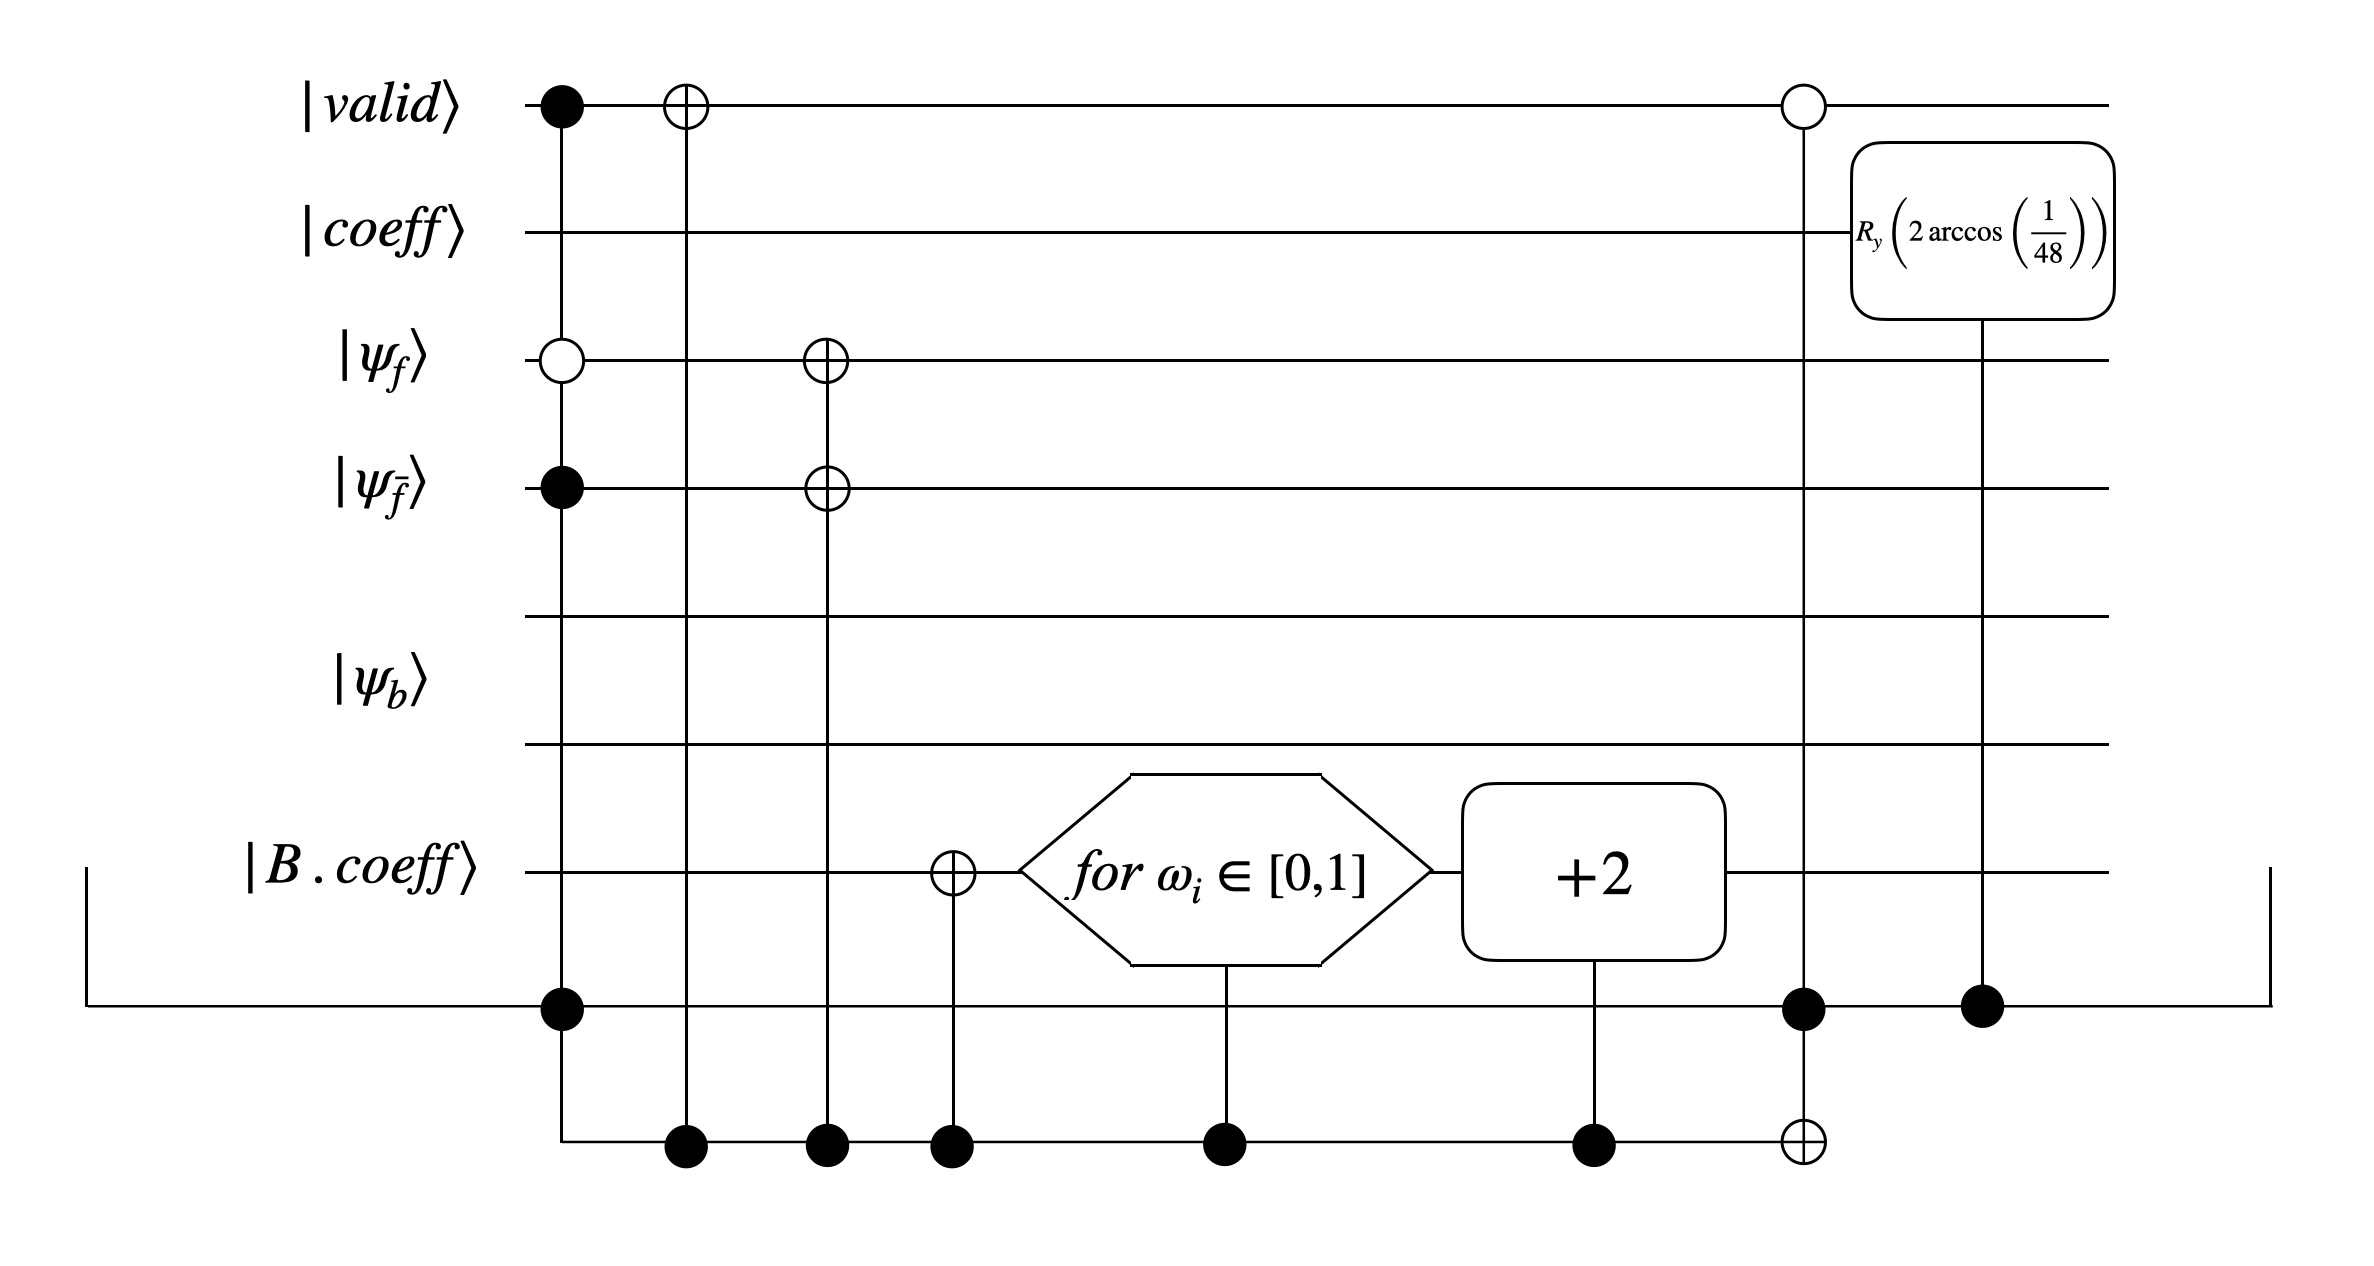
\includegraphics[width = 0.7\linewidth]{figures/T0.png}
    \caption{\textit{Select} unitary $U_{T_0}$ that block-encodes $T_0 = b_0^\dagger d_0(a_0^\dagger)^2$}
\end{figure}
\begin{figure}[h]
    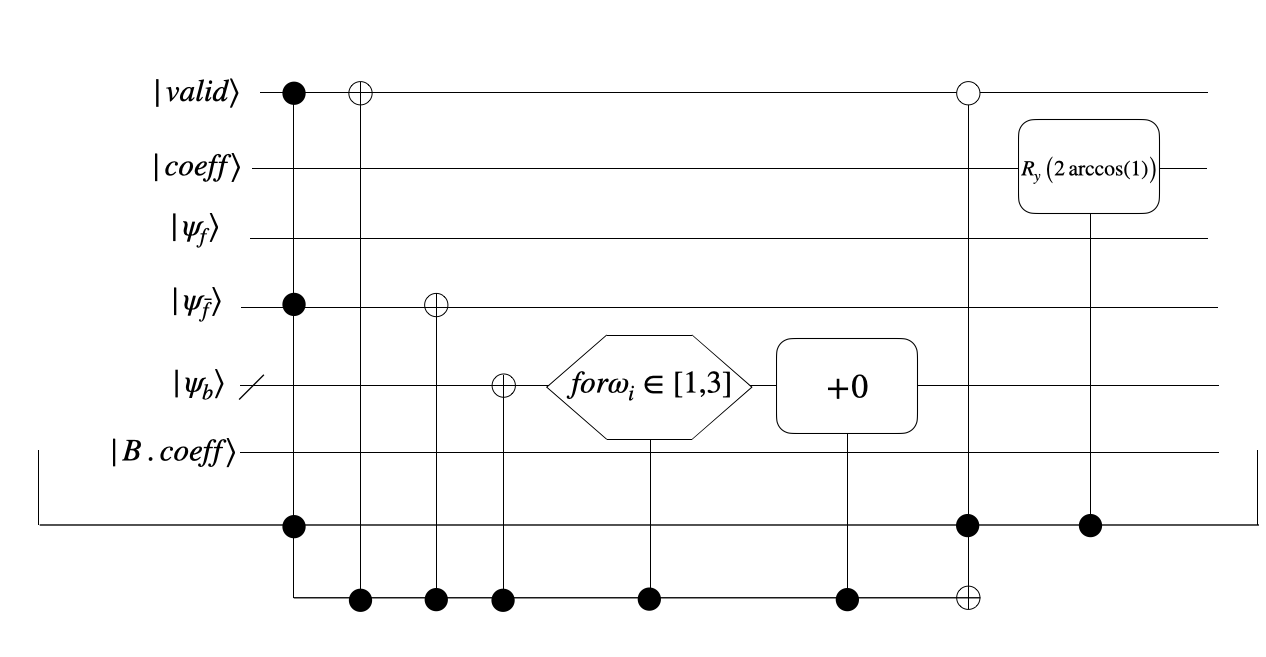
\includegraphics[width = 0.7\linewidth]{figures/T1.png}
    \caption{\textit{Select} unitary $U_{T_1}$ that block-encodes $T_1 = a_0^\dagger a_0 d_0^\dagger$}
\end{figure}
\begin{figure}[h]
    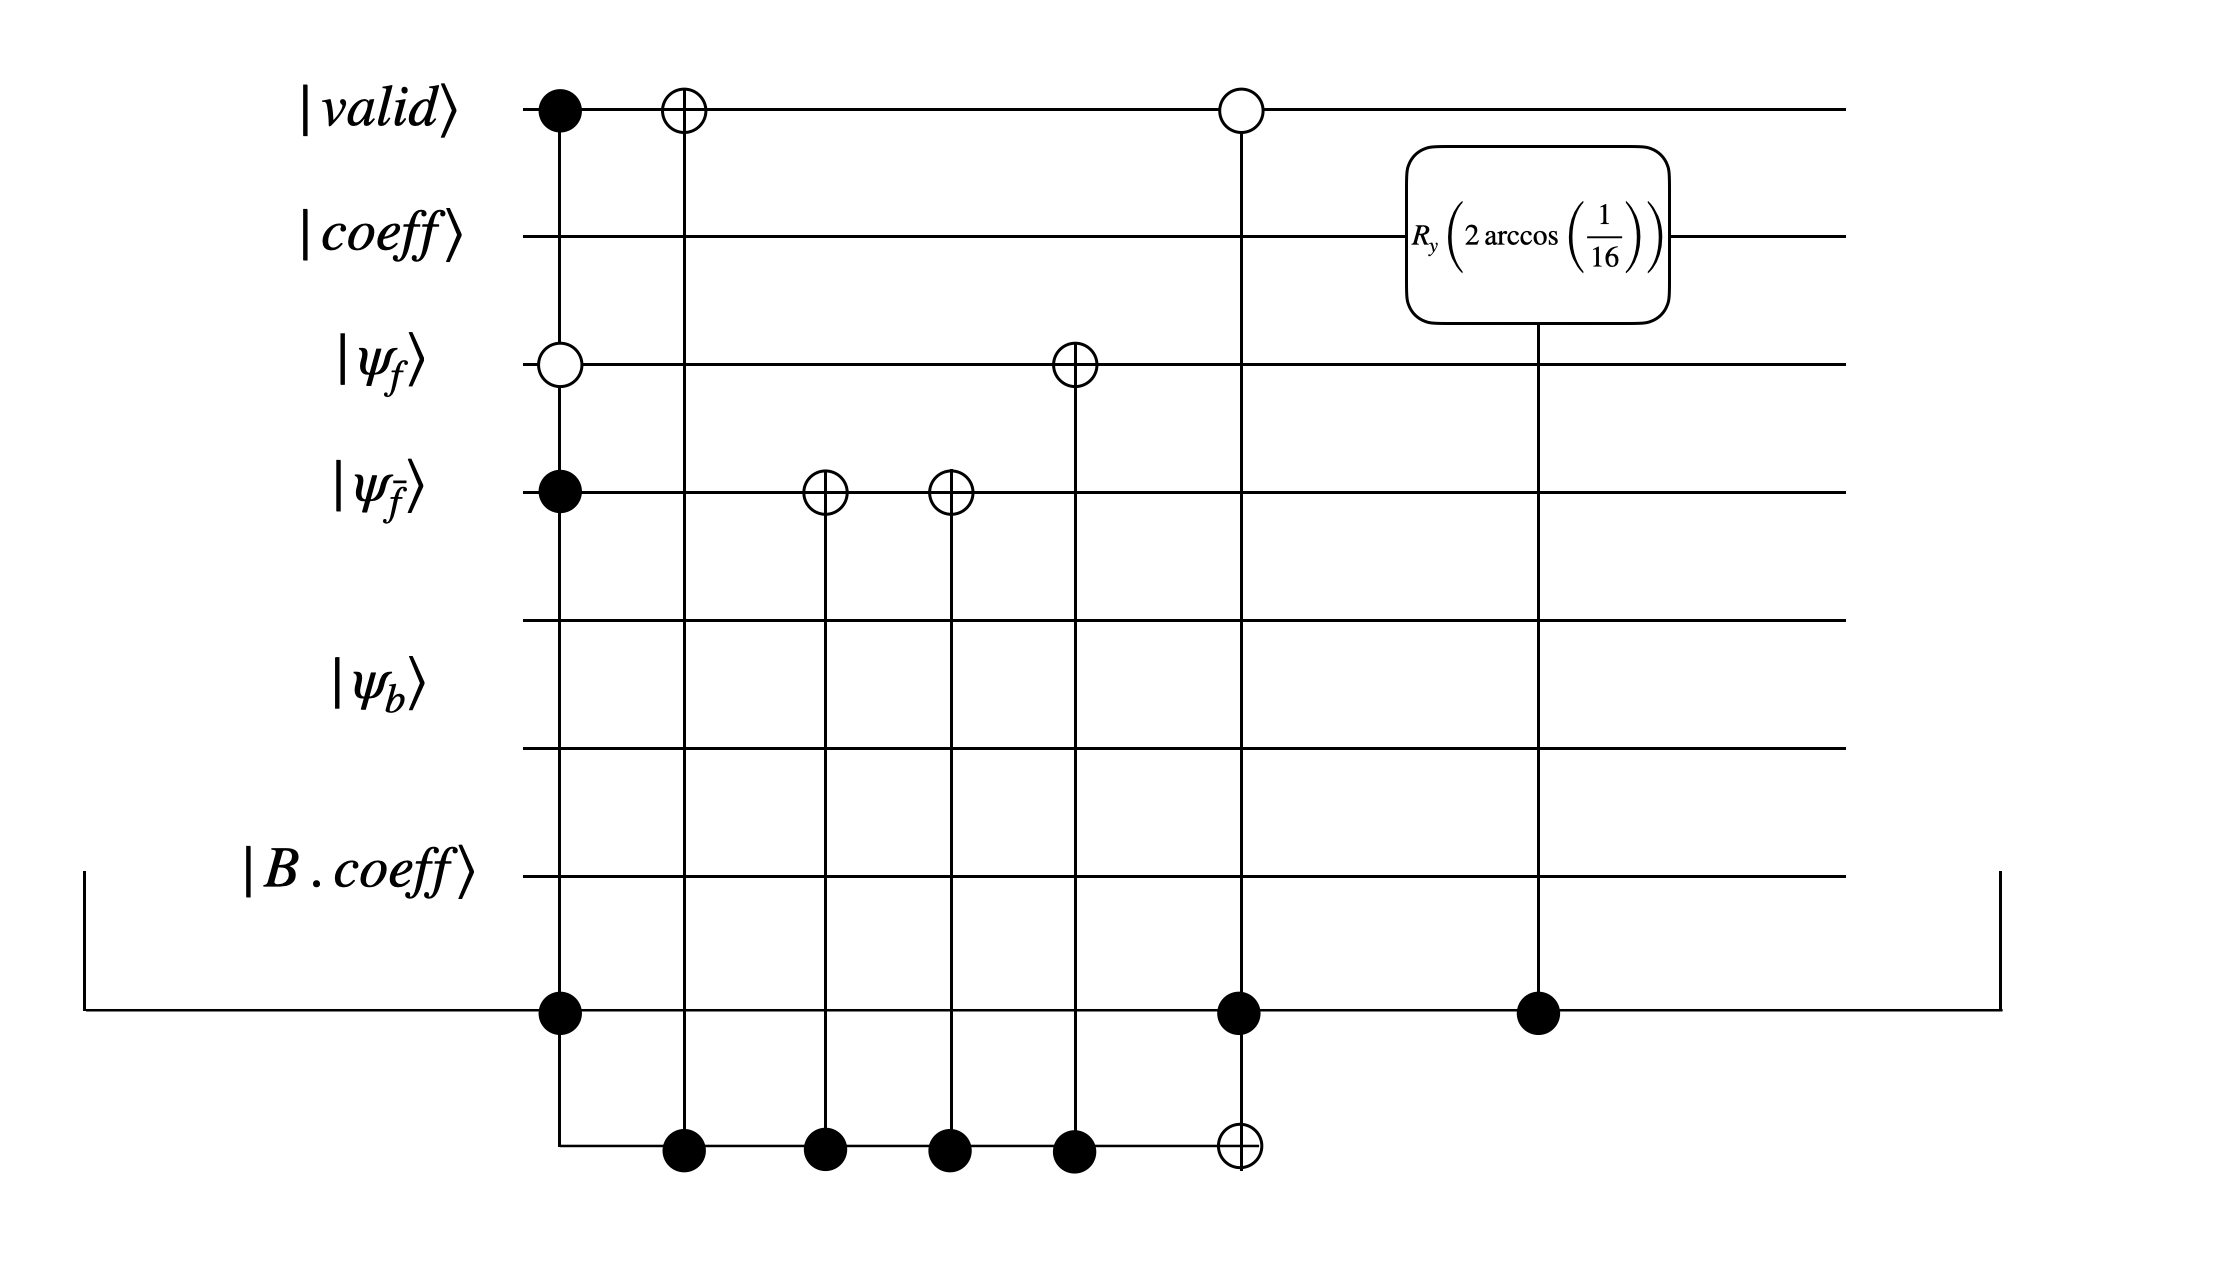
\includegraphics[width = 0.7\linewidth]{figures/T2.png}
    \caption{\textit{Select} unitary $U_{T_2}$ that block-encodes $T_2 = b_0^\dagger d_0^\dagger d_0$}
\end{figure}

\textbf{Step 4: Count gates:} Using the notation in \ref{count gates not.}, the preceeding three unitaries have the following gate counts:

\begin{align}
    C_{U_{T_0}} &= (8, 7, 8)\\
    C_{U_{T_1}} &= (7, 6, 8)\\
    C_{U_{T_2}} &= (4, 3, 2)
\end{align}
When we add in the cost of the controlled multiplexor over the index register, we add two more left and right elbows ($N_{elbows} = L - 1$, where $L$ is the number of terms). Thus, the total cost of the \textit{select} oracle is $C_{\textit{select}} = (21, 18, 18)$. 

To get the total circuit cost, the \textit{prepare} oracle cost must be included. \textit{USP} doesn't have a cost since it is just Haddamards, thus $C^{\text{USP}}_{\text{prepare}} = (0, 0, 0)$; however, \textit{ASP} does incrue an additional arbitrary rotation cost: $C_{\text{prepare}}^{\text{ASP}} = (0, 0, 3)$. 

Thus, the total cost to block encode the Hamiltonian \ref{ex} is $C^{\text{USP}} = (21, 18, 18)$ or $C^{\text{ASP}} = (21, 18, 24)$.

\textbf{Step 5: Post-process the eigenvalues:} After obtaining the full block-encoding of the Hamiltonian, the eigenvalues (which can be obtained via phase estimation) must be post-processed. This is because the eigenvalues of the block encoded Hamiltonian will correspond to $H^*$, \textit{not} $H$ (the original problem Hamiltonian).
The final scaling of the Hamiltonian that needs to be post-processed is given in equation \ref{post-process}. $(\Omega + 1)^{K / 2}$ is the same for \textit{USP} and \textit{ASP}; however, the additional scaling factor $\lambda$ will change $H^*$, depending on the preparation protocol. It is easy to calculate $(\Omega + 1)^{K/2} = 4^{2/2}$, and we obtained $\lambda_{usp} = 8$ and $\lambda_{asp} = 3.75$ in step 3. 
We then can get $H^*_{\text{USP}} = \frac{H}{32}$, and $H^*_{\text{ASP}} = \frac{H}{15}$. Thus, $E_{USP} = 32E^*_{USP}$ and $E_{ASP} = 15E^*_{ASP}$.